\documentclass[a4paper]{article}
\usepackage[utf8]{inputenc} % - Defines what coding LaTeX uses. Use this one.
\usepackage{float}
\usepackage[swedish]{babel}
\usepackage{graphicx}
\graphicspath{ {./images/} }

\title{Sprint 4 - Slutrapport \\ 
\large{Laboration för D0018E - Databasteknik}}

\author{Josef Utbult \\
{\tt josutb-7@student.ltu.se}}
\date{\today}

\begin{document}

\pagenumbering{roman}
\maketitle
\newpage
\tableofcontents

\section{Introduktion}
Det här är en webbshop utvecklad för en laboration i kurset \textit{D0020E}. \textit{Musikdong}, som är webbshopens namn, säljer gitarrpedaler, fullt legala tjänster samt annat smått och gott. Nu är sidan färdig och sitter sidan uppe på IP-adressen \texttt{http://130.240.200.51:5000}. Servern är aktiv om man ber Josef att sätta på den, annars ligger den passiv.

\section{Executive summary}
\pagenumbering{arabic}
\subsection{Sprint 1 - Josef}
Jag har jobbat med att sätta upp servern inför Sprint 1. Vi använde den virtuella maskinen tillhandahållen av LUDD, där vi satt upp mySql som databas, en flask-applikation för att kommunicera med backenden samt Nginx för att komma åt sidan via vår statiska IP.

Jag har även experimenterat med att interagera med mySql, främst på min egen maskin för enkelhetens skull, men sett till så att allt är kompatibelt för att emigrera till den virtuella maskinen.

\subsection{Sprint 1 - Leo}
Jag har tillsammans med Josef tagit fram user stories samt gjort en enkel hemsida med html och css. 

\subsection{Sprint 2 - Josef}
Jag har byggt om databasen för att hantera produkter, kategorier och användare m.m. Jag har även lagt till strukturen för orderhantering i databasen, i form av ett orders-table och ett orderItem-table. En grundläggande manager-sida har också lagts till.

\subsection{Sprint 3 - Josef}
Jag har byggt klart manager-sidan med möjlighet att lägga till produkter och kategorier, samt redigera användare, produkter och kategorier. Jag har fixat orderhanteringen och implementerat att priset låses efter att ordern läggs. Jag har även implementerat reviws. 

\subsection{Sprint 4 - Josef}
Jag har lagt till en sökbar i headern som söker på produktnamn.

\newpage
\section{Userstories}
\subsection{Admin}
\begin{enumerate}
  \item Har alla rättigheter som manager.
  \item Kan ändra rättigheter för alla användare på sidan.
  \item Kan lägga till och radera
  %
  \begin{itemize}
    \item Kategorier
    \item Tagtyper
  \end{itemize}
\end{enumerate}
%
\subsection{Manager}
\begin{enumerate}
  \item Har alla rättigheter som en inloggad användare.
  \item Kan öppna en manager meny.
  \item Har tillgång till att redigera alla
  %
  \begin{itemize}
    \item Användare
    \item Produkter
    \item Kategorier 
    \item Tagtyper
    \item Reviews
    \item Carts
    \item Orders
  \end{itemize}
  %
  \item Kan få en lista med alla ordrar i manager-menyn, där man ser betalade ordrar samt hanterade ordrar separat.
  \item Kan lägga till och radera
  \begin{itemize}
  \item Användare
  \item Produkter
  \end{itemize}
\end{enumerate}
%
\subsection{Inloggad användare}
\begin{enumerate}
  \item Har alla rättigheter som en icke inloggad användare.
  \item Kan lägga produkter i sin kundvagn.
  \item Kan lägga en review på en produkt.
  \item Kan öppna sin kundvagn och se vad som ligger i.
  \item Kan lägga en order som senare hanteras av managers.
  \item Kan logga ut från sin användare.
\end{enumerate}
%
\subsection{Icke inloggad användare}
\begin{enumerate}
  \item Kan orientera sig mellan kategorier till produkter.
  \item Kan använda sökbaren för att söka på ett produktnamn.
  \item Kan logga in, eller skapa en användare.
\end{enumerate}
%
\section{Nuvarande Backlog}
Backlogen ligger i form av issues på Josefs github. \texttt{https://github.com/JosefUtbult/Musikdong}.
%
\begin{figure}[H]
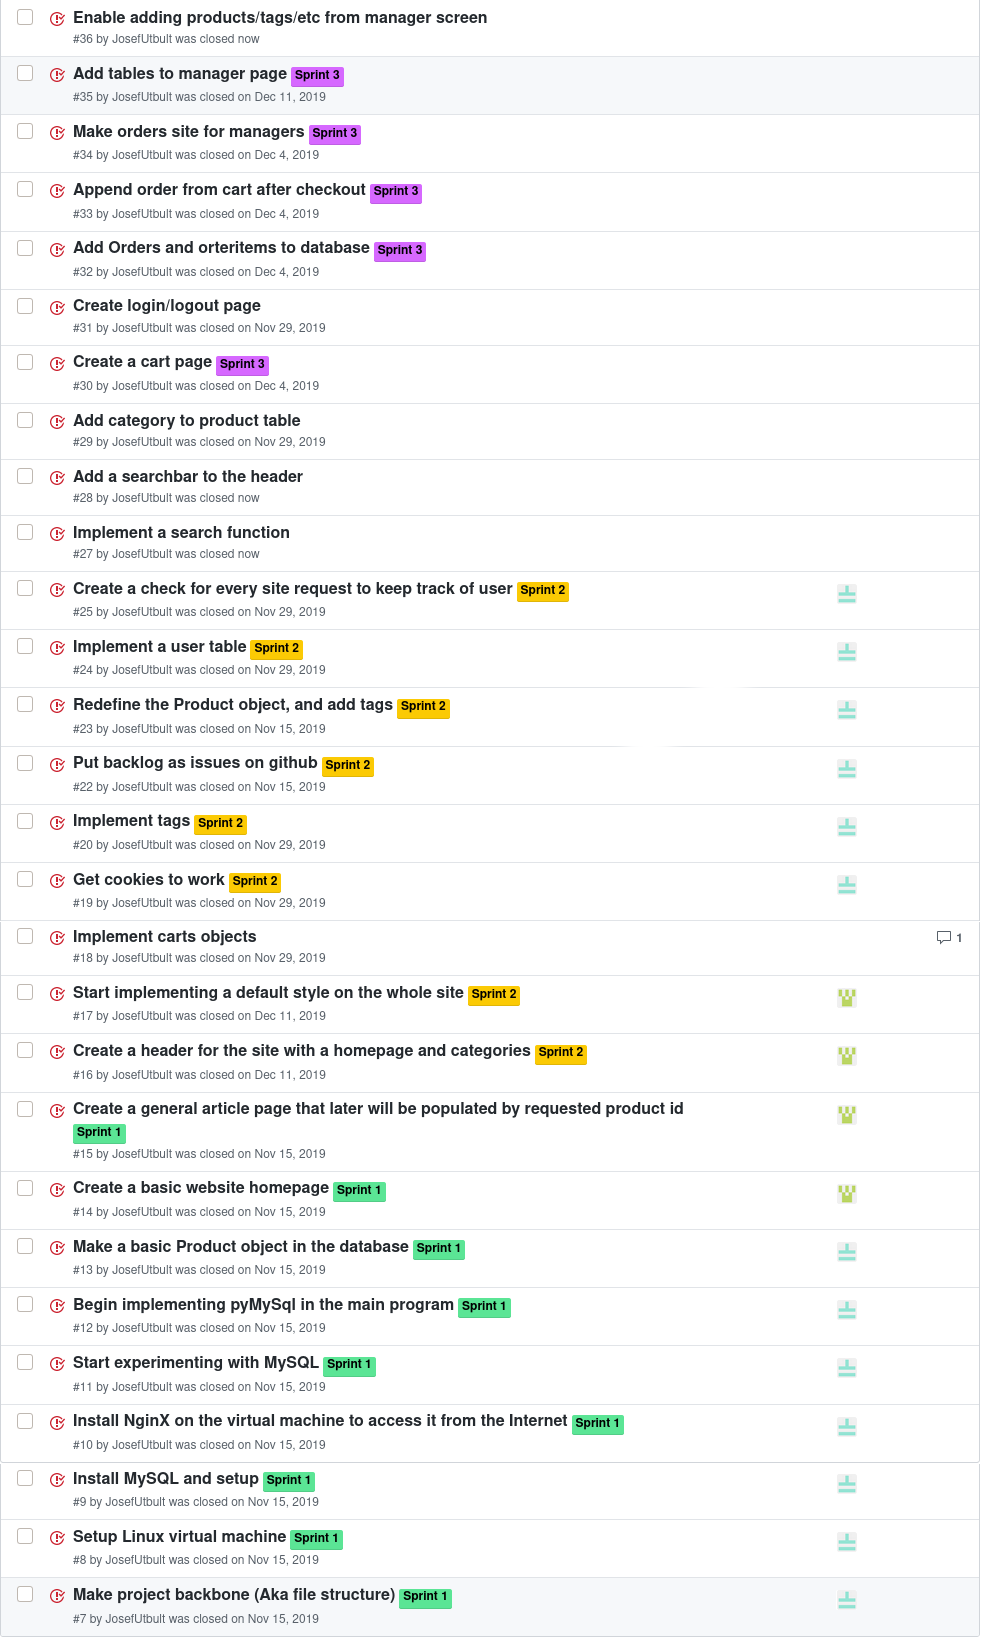
\includegraphics[width=\textwidth,height=\textheight,keepaspectratio]{Backlog.png}
\centering
\end{figure}
%
\section{ER-diagram}
\begin{figure}[H]
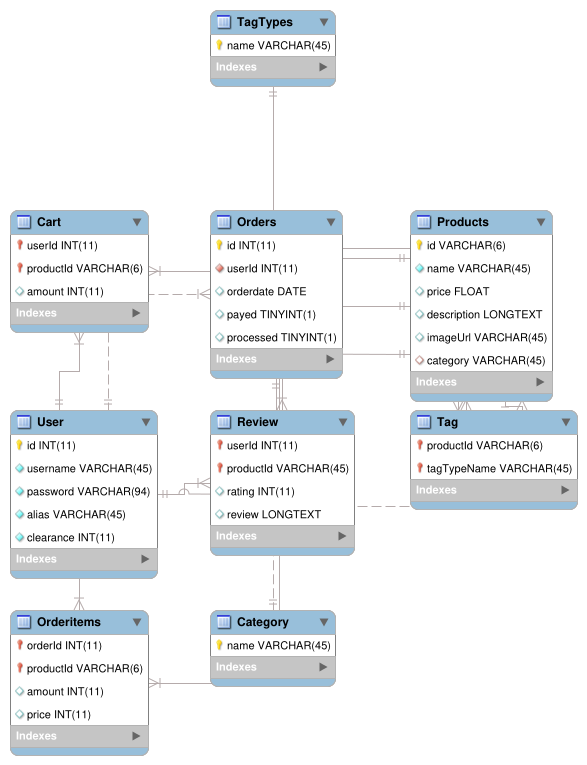
\includegraphics[width=\textwidth,height=\textheight,keepaspectratio]{ER.png}
\caption \newline ER-diagram taget från \textit{Mysql Workbench}.
\centering
\end{figure}
%
\section{Kodbas}
Koden för projektet finns tillgänglig publikt på Github under Josefs användare (JosefUtbult). Där ligger även backloggen i form av issues. \\
\texttt{https://github.com/JosefUtbult/Musikdong/}
%
\section{Tester}
\subsection{Icke inloggad användare}
\subsubsection{Hitta en produkt}
\begin{enumerate}
  \item Öppna startsida.
  \item Navigera till en kategori.
  \item Navigera till en produkt.
  \item Öppna sida för produkt.
\end{enumerate}
%
\subsubsection{Sök efter produkt}
\begin{enumerate}
  \item Navigera till sökbaren.
  \item Skriv in namn eller del av namn på en produkt.
  \item Tryck på \textit{Sök}.
  \item Välj produkt bland resultaten.
\end{enumerate}
%
\subsubsection{Skapa användare}
\begin{enumerate}
\item Tryck på \textit{Sign Up}.
\item Välj ett användarnamn.
\begin{itemize}
  \item Det ska inte gå att välja ett användarnamn som redan är registrerad.
\end{itemize}
\item Välj lösenord.
\item Skapa användare.
\end{enumerate}
%
\subsubsection{Logga in}
\begin{enumerate}
  \item Tryck på \textit{Login}.
  \item Skriv in användarnamn och lösenord.
  \item Logga in.
\end{enumerate}
%
\subsection{Inloggad användare}
\subsubsection{Lägg vara i kundvagn}
\begin{enumerate}
  \item Navigera till en vara.
  \item Lägg i kundvagn.
\end{enumerate}
%
\subsubsection{Visa kundvagn}
\begin{enumerate}
  \item Tryck på kundvagn i headern.
\end{enumerate}
%
\subsubsection{Lägg order}
\begin{enumerate}
  \item Öppna kundvagnen.
  \item Lägg order.
\end{enumerate}
%
\subsubsection{Lägg review}
\begin{enumerate}
  \item Navigera till en produkt.
  \item Använd slidern för att ställa in ett betyg mellan ett till fem.
  \item Skriv en review.
  \item Tryck på \textit{review}.
\end{enumerate}
%
\subsection{Manager}
\subsubsection{Visa produkt/användare/ordrar}
\begin{enumerate}
  \item Tryck på \textit{Manager} i headern.
  \item Navigera till produkt/användare/ordrar
  \item Öppna sida för produkt/användare/ordrar
\end{enumerate}
%
\subsubsection{Redigera produkt/användare/ordrar}
\begin{enumerate}
  \item Navigera till produkt/användare/ordrar
  \item Redigera produkt/kategori/ordrar
  \item Tryck på \textit{Update}
\end{enumerate}
%
\subsubsection{Lägga till produkt}
\begin{enumerate}
  \item Öppna \textit{Manager}.
  \item Tryck på \textit{Add}.
  \item Fyll i produkt.
  \item Tryck på \textit{Add}.
\end{enumerate}
%
\subsubsection{Radera produkt/användare/ordrar}
\begin{enumerate}
  \item Navigera till produkt/användare/ordrar.
  \item Redigera produkt/användare/ordrar.
  \item Tryck på \textit{Delete}.
\end{enumerate}
%
\subsection{Admin}
\subsubsection{Updatera kategori/rättigheter}
\begin{enumerate}
  \item Utförs på samma sätt som produkt/användare/ordrar.
\end{enumerate}
%
\subsubsection{Radera kategor}
\begin{enumerate}
  \item Utförs på samma sätt som produkt/användare/ordrar.
\end{enumerate}
%
\section{Limitations}
\subsection{Säkerhet}
Sidan inkluderar en sökbar som skickar ett sök-request till servern. Detta request hanteras av Pymysqls inbyggda formatering av requests, men utöver det görs ingen säkerhetscheck på indatan. Detta kan i teorin släppa igenom vissa SQL-injektioner.
%
\subsection{Review}
En användare kan endast lägga en review per produkt. Detta då databasen använder en tuple av \textit{userId} och \textit{productId} som primär nyckel samt att GUIn bygger på att man kan lägga en review och senare kan redigera denna. Huruvida detta är att föredra går att diskutera, men detta är hur det har implementerats i projektet.
%
\subsection{Taggar}
Taggar samt taggtyper var en ide för att möjliggöra en sökfunktion. Detta finns färdigt i databasen, men implementationen blev nedprioriterat. Tanken från början var att taggar skulle inkluderas i sökresultaten då en användare använder sökbaren, men denna implementationen nedprioriterades tills den inte lägre var väsentlig för projektet.
%
\subsection{Produktbilder}
URL för bilder på produkter finns tillagt i databasen, men tillägning av bilder, lagring samt visning av bilder på produktsidor blev inte implementerat i programmet.
%
\end{document}
%
